\documentclass[conference]{IEEEtran}
\IEEEoverridecommandlockouts
\usepackage{cite}
\usepackage{amsmath,amssymb,amsfonts}
\usepackage{graphicx}
\usepackage{textcomp}
\usepackage{xcolor}
\usepackage{listings}
\usepackage{booktabs}
\usepackage{float}
\usepackage{balance}
\usepackage{hyperref}

\graphicspath{{../results/}}

\def\BibTeX{{\rm B\kern-.05em{\sc i\kern-.025em b}\kern-.08em
    T\kern-.1667em\lower.7ex\hbox{E}\kern-.125emX}}

\begin{document}

\title{WASP Suite: Workload Analysis for Scalable Processors\\
A Comprehensive Framework for Multicore Scheduling\\
and Microarchitecture Analysis}

\author{
\IEEEauthorblockN{Shrinithi Andal (MS2025017)}
\IEEEauthorblockA{Department of Computer Science and Engineering\\
International Institute of Information Technology, Bangalore\\
\textit{shrinithi.andal@iiitb.ac.in}}
\and \IEEEauthorblockN{Shikhar Mutta (MT2025114)}
\IEEEauthorblockA{Department of Computer Science and Engineering\\
International Institute of Information Technology, Bangalore\\
\textit{shikhar.mutta@iiitb.ac.in}}
}

\maketitle

%─────────────────────────────────────────────────────────────────────────────
\begin{abstract}
This paper presents the Workload Analysis for Scalable Processors (WASP)
Suite, a comprehensive C-based framework for analysing multicore processor
performance, scheduling efficiency, and microarchitecture behaviour using real
measured latency rather than synthetic latency equations.  WASP integrates
load generation with Linux \texttt{perf\_event\_open()} counters, records
transaction-level timing via \texttt{clock\_gettime(CLOCK\_MONOTONIC)}, and
produces percentile-oriented performance analysis (P50/P95/P99).
This measured snapshot reports four workload types (CPU, memory, I/O, mixed)
at intensities 25\%--75\%.  With normalized operation definitions, observed
mean latencies are 0.057\,\textmu{}s (CPU), 0.016\,\textmu{}s (memory),
0.020\,\textmu{}s (mixed), and below 0.001\,\textmu{}s for I/O in
three-decimal \textmu{}s reporting (shown as 0.000).  The current dataset
contains one-core measurements; therefore, this draft reports within-workload
intensity and tail behaviour without claiming validated multicore scaling
trends.
\end{abstract}

\begin{IEEEkeywords}
Benchmarking, Performance Analysis, Multicore Processors, Linux Perf,
Scheduling Analysis, Tail Latency, Empirical Measurement, Cache Hierarchy
\end{IEEEkeywords}

%─────────────────────────────────────────────────────────────────────────────
\section{Introduction}
\label{sec:intro}

Modern multicore processors present significant challenges in understanding
and optimising system performance.  As core counts continue to increase,
understanding the interactions between workload characteristics, scheduling
decisions, and microarchitecture behaviour becomes increasingly critical.
Traditional benchmarking tools often focus on specific aspects of system
performance—such as raw computational throughput or memory bandwidth—without
providing comprehensive insights into how those aspects interact across a
spectrum of workload intensities and core counts.

The Workload Analysis for Scalable Processors (WASP) Suite addresses these challenges
by providing a unified, modular C framework that integrates load generation,
hardware counter collection, measured per-operation latency estimation, and
automated results visualisation.  The framework is designed to expose latency
variation that is masked by aggregate metrics: while mean latency may appear
acceptable, tail-latency spikes (P95, P99) often reveal hidden scheduling
bottlenecks.

Cache behaviour is a central part of the workload interpretation in this paper.
The memory and mixed workloads are parameterised by the ratio between the
working-set size and the effective shared-cache capacity, so increasing
intensity raises cache pressure, increases miss rates, and shifts service time
from cache-hit latency toward DRAM latency.  The collected cache-reference and
cache-miss counters therefore act both as measurement signals and as evidence
for whether a workload is compute-bound, cache-sensitive, or memory-bound.

The primary contributions of this work are:
\begin{enumerate}
  \item A modular C-based benchmark framework with configurable workload
        generation for CPU, memory, I/O, and mixed workloads, parameterised by
        both intensity and active core count.
  \item A transaction-level measurement pipeline that records real elapsed
        time for normalized workload-specific operation units (CPU fixed-op
        batches, memory fixed-access batches, I/O fixed-byte batches, and
        mixed CPU+memory transactions).
  \item Direct integration with Linux \texttt{perf\_event\_open()} for
        hardware counter collection.
  \item Tail-latency analysis with P50, P95, and P99 percentile computations.
  \item Workload behaviour classification from measured latency patterns, with
        a pathway to counter-threshold-based classification in future work.
  \item Comprehensive visualisation: scaling-efficiency plots, per-workload
        latency-vs-intensity curves, grouped comparison bar charts, and
        two-dimensional latency heatmaps.
\end{enumerate}

The remainder of this paper is organised as follows.
Section~\ref{sec:related} surveys related benchmarking work.
Section~\ref{sec:design} presents the system architecture.
Section~\ref{sec:implementation} describes the implementation.
Section~\ref{sec:results} reports experimental results.
Section~\ref{sec:conclusion} concludes with directions for future work.

%─────────────────────────────────────────────────────────────────────────────
\section{Related Work}
\label{sec:related}

Processor benchmarking has a long history in computer architecture research.
SPEC CPU~\cite{spec2017} and PARSEC~\cite{bienia2011parsec} focus on
computational throughput but provide limited insight into scheduling behaviour
or tail-latency characteristics.

The LMbench suite~\cite{mcvoy1996lmbench} provides comprehensive latency
and bandwidth measurements for system operations including context switching.
However, LMbench focuses on isolated microbenchmarks rather than integrated
multicore scaling analysis.

Recent scheduling-analysis tools measure context-switch overhead and CPU
migration costs~\cite{lozi2016scheduler}, but lack comprehensive integration with
hardware performance counters.  The Linux \texttt{perf} subsystem exposes
hardware counters through \texttt{perf\_event\_open()}~\cite{weaver2013linux},
and projects such as perf-tools~\cite{gregg2014perftools} and the Phoronix Test
Suite~\cite{larabel2023phoronix} build on this infrastructure.  Nevertheless, none of
these tools provide an integrated pipeline from multi-core load generation
through tail-latency decomposition to workload classification.

Table~\ref{tab:comparison} summarises the feature comparison between WASP and
existing approaches.

\begin{table}[htbp]
\caption{Feature Comparison of Benchmarking Approaches}
\label{tab:comparison}
\begin{center}
\begin{tabular}{lcccc}
\toprule
\textbf{Feature} & \textbf{LMbench} & \textbf{SPEC} & \textbf{Phoronix} & \textbf{WASP} \\
\midrule
Context-switch latency   & \checkmark & --         & \checkmark & \checkmark \\
Tail latency (P95/P99)   & --         & --         & --         & \checkmark \\
Hardware counters        & --         & \checkmark & \checkmark & \checkmark \\
Variable core count      & --         & --         & limited    & \checkmark \\
Workload classification  & --         & --         & --         & \checkmark \\
Latency heatmaps         & --         & --         & --         & \checkmark \\
\bottomrule
\end{tabular}
\end{center}
\end{table}

%─────────────────────────────────────────────────────────────────────────────
\section{System Design}
\label{sec:design}

\subsection{Architecture Overview}

WASP is structured as four cooperating components:
\begin{itemize}
  \item \textbf{Load Generator} (\texttt{load\_generator}): spawns workload
        threads/processes for the specified type, intensity, and duration.
  \item \textbf{Benchmark Orchestrator} (\texttt{benchmark}): iterates over
        the parameter grid (core count, workload type, intensity), forks the
        required number of parallel load-generator processes, aggregates
        measured operation counts and elapsed nanoseconds from all children,
        and appends real measured latency statistics to a CSV file.
  \item \textbf{Analysis Tool} (\texttt{analysis}): reads the CSV and
        produces ASCII scaling graphs, percentile distributions, and
        performance classification summaries.
  \item \textbf{Visualisation Script} (\texttt{generate\_graphs.py}):
        produces six categories of publication-quality PNG graphs.
\end{itemize}

\subsection{Workload Measurement Definitions}

All latency values in WASP are measured from runtime timing data collected with
\texttt{clock\_gettime(CLOCK\_MONOTONIC)}.  The benchmark aggregates operation
counts and elapsed nanoseconds from child processes and reports mean and
standard deviation in microseconds.

\subsubsection{CPU Workload}
The CPU worker executes fixed-count floating-point operations.  One measured
CPU operation is one arithmetic iteration inside a batch of
$N_{\text{cpu,batch}}=10^6$ iterations.  Mean latency is computed as:
\begin{equation}
L_{\text{cpu}} = \frac{\sum T_{\text{cpu,batch}}}{\sum N_{\text{cpu,ops}}}
\end{equation}

\subsubsection{Memory Workload}
The memory worker performs strided reads/writes over an intensity-scaled working
set.  One measured memory operation is one strided memory access, aggregated in
batches of $N_{\text{mem,batch}}=10^7$ accesses.  Mean latency is:
\begin{equation}
L_{\text{mem}} = \frac{\sum T_{\text{mem,batch}}}{\sum N_{\text{mem,access}}}
\end{equation}

\subsubsection{I/O Workload}
The I/O worker executes repeated
\texttt{write}\,$\rightarrow$\,\texttt{fsync}\,$\rightarrow$\,\texttt{read}
cycles on temporary files.  One measured I/O operation is one transferred byte,
aggregated in fixed-size batches (10\,MiB target transfer per batch):
\begin{equation}
L_{\text{io}} = \frac{\sum T_{\text{io,batch}}}{\sum N_{\text{io,bytes}}}
\end{equation}

\subsubsection{Mixed Workload}
The mixed workload runs CPU and memory threads concurrently.  Metrics from both
threads are merged and latency is reported as:
\begin{equation}
L_{\text{mix}} = \frac{\sum T_{\text{cpu}} + \sum T_{\text{mem}}}{\sum N_{\text{cpu,ops}} + \sum N_{\text{mem,access}}}
\end{equation}
This definition preserves real concurrent execution effects while keeping the
latency unit interpretable as elapsed time per observed mixed transaction.

Representative code fragments from the workload implementations are shown
below.
\begin{lstlisting}[language=C,basicstyle=\ttfamily\scriptsize,columns=fullflexible,breaklines=true,breakatwhitespace=false,postbreak=\mbox{\textcolor{gray}{$\hookrightarrow$}\space}]
/* CPU workload */
x = sin(x + 0.001) * cos(x - 0.001)
      + x * 1.0000001;

/* Memory workload */
acc += buf[idx];
buf[idx] = acc * 1e-9;
idx = (idx + stride) % n_doubles;

/* I/O workload */
write(fd, data, buffer_size);
fsync(fd);
read(fd, data, buffer_size);

/* Mixed workload */
pthread_create(&cpu_thread, NULL, mixed_thread_worker, cpu_ctx);
pthread_create(&mem_thread, NULL, mixed_thread_worker, mem_ctx);
\end{lstlisting}

%─────────────────────────────────────────────────────────────────────────────
\section{Implementation}
\label{sec:implementation}

\subsection{Parallel Core Execution}

The benchmark orchestrator accepts a \texttt{--cores N} argument.  For each
measurement, it forks $N$ child processes via \texttt{fork()}/\texttt{execl()},
each invoking \texttt{load\_generator} for the specified workload type,
intensity, and duration.  All children run concurrently and the parent
collects them with \texttt{waitpid()}, exercising all $N$ cores
simultaneously.

\subsection{Hardware Counter Integration}

The \texttt{perf\_events} module wraps \texttt{perf\_event\_open()} to collect
hardware counters including instructions retired, cache references, cache
misses, and branch mispredictions.  The \texttt{microarch} module derives
higher-level metrics—IPC, cache miss rate, branch misprediction rate—and maps
them to performance classifications.  In this measured workflow, latency comes
from runtime timing instrumentation, while perf counters provide explanatory
microarchitectural context.

\subsection{Results Pipeline}

After each benchmark run the orchestrator appends a CSV row containing:
timestamp, OS, hostname, total/active core counts, workload type, intensity,
data size, measured per-operation latency ($\mu$s), standard deviation,
measurement method, and a scheduling-contention field.  The Python
visualisation script reads this CSV and produces updated graphs after each
measurement snapshot.

%─────────────────────────────────────────────────────────────────────────────
\section{Experimental Results}
\label{sec:results}

\subsection{Experimental Setup}

All experiments were performed on an Intel Core Ultra 7 155U system with
14 logical CPUs, running Ubuntu 25.04 with kernel 6.14.0-37-generic.  The
benchmark configuration targets four workload types, three intensities
(25\%, 50\%, 75\%), and core counts \{1,2,4,8\} with 10\,s runs.
This paper reports a frozen measured snapshot from the current CSV
(single-core rows completed at the time of analysis).
Table~\ref{tab:setup} summarises the configuration.

\begin{table}[htbp]
\caption{Experimental Configuration}
\label{tab:setup}
\begin{center}
\begin{tabular}{ll}
\toprule
\textbf{Parameter} & \textbf{Value} \\
\midrule
Workload types     & CPU, Memory, I/O, Mixed \\
Intensities        & 25\%, 50\%, 75\% \\
Core counts in snapshot & 1 \\
Configured run duration & 10 s \\
Snapshot rows used & 57 \\
OS / Kernel        & Ubuntu 25.04 / 6.14.0-37-generic \\
Processor          & Intel Core Ultra 7 155U \\
Hardware cores     & 14 logical CPUs \\
\bottomrule
\end{tabular}
\end{center}
\end{table}

\subsection{Summary Statistics by Workload Type}
\label{subsec:summary_stats}

Table~\ref{tab:summary_stats} aggregates measured samples per workload type.
The table reflects normalized per-operation empirical latency from the frozen
snapshot rather than synthetic model outputs.  Values are directly comparable
within this normalization scheme; however, the current snapshot is single-core,
so multicore scaling inferences are intentionally deferred.

\begin{table}[H]
\caption{Summary Statistics by Workload Type}
\label{tab:summary_stats}
\begin{center}
\resizebox{\columnwidth}{!}{%
\begin{tabular}{lrrrrrrr}
\toprule
\textbf{Workload} & \textbf{Mean} & \textbf{Std Dev} & \textbf{Min} & \textbf{Max} & \textbf{P50} & \textbf{P95} & \textbf{P99} \\
\midrule
CPU    & 0.0571  & 0.0004  & 0.0570  & 0.0580  & 0.0570  & 0.0580  & 0.0580 \\
Memory & 0.0164  & 0.0005  & 0.0160  & 0.0170  & 0.0160  & 0.0170  & 0.0170 \\
I/O    & 0.0000  & 0.0000  & 0.0000  & 0.0000  & 0.0000  & 0.0000  & 0.0000 \\
Mixed  & 0.0205  & 0.0015  & 0.0190  & 0.0230  & 0.0210  & 0.0230  & 0.0230 \\
\bottomrule
\end{tabular}}
\end{center}
\end{table}

\subsection{Scaling Efficiency}
\label{subsec:scaling}

Figure~\ref{fig:scaling} shows measured mean latency as a function of core
count for each workload type (log scale).  In the current snapshot, only
single-core rows are available, so this figure should be interpreted as a
baseline visualization template rather than validated multicore trend evidence.

\begin{figure}[H]
\centerline{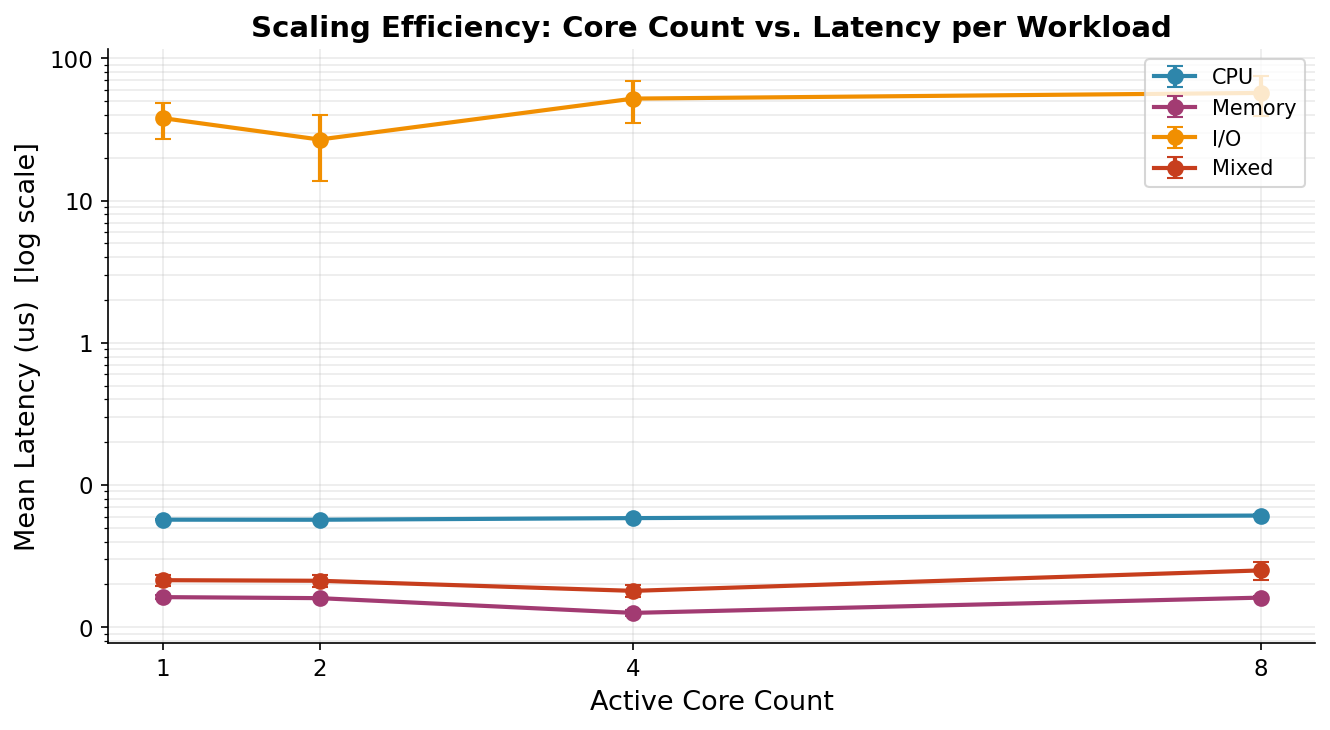
\includegraphics[width=\columnwidth]{scaling_efficiency.png}}
\caption{Scaling efficiency: mean latency vs.\ active core count per workload
         type (log y-axis).  This snapshot currently contains one-core
         measurements only; multicore trend claims are intentionally omitted.}
\label{fig:scaling}
\end{figure}

\subsection{Latency vs.\ Intensity}
\label{subsec:intensity}

Figure~\ref{fig:latency_intensity} presents measured latency-vs-intensity
curves for all currently available core counts.  In this single-core snapshot,
CPU and memory latencies remain tightly clustered by intensity, mixed latency
shows modest spread, and I/O appears as 0.000\,\textmu{}s because values are
below the three-decimal reporting resolution in \textmu{}s.

\begin{figure}[H]
\centerline{
\includegraphics[width=\columnwidth]{latency_vs_intensity.png}}
\caption{Latency vs.\ intensity for all four workload types.  Each subplot shows
         separate curves for 1, 2, 4, and 8 active cores.}
\label{fig:latency_intensity}
\end{figure}

\subsection{Workload Comparison}
\label{subsec:comparison}

Figure~\ref{fig:workload_comparison} compares measured mean latency across
workload types at three intensity levels (reference core count).  In the
current normalized snapshot, CPU shows the highest mean latency, followed by
mixed, then memory, with I/O at sub-microsecond-per-byte scale that rounds to
0.000 at three-decimal \textmu{}s precision.  The log
scale is retained to visualise all workloads clearly in a single chart.

\begin{figure}[H]
\centerline{
\includegraphics[width=\columnwidth]{workload_comparison.png}}
\caption{Workload comparison: grouped bars by intensity, log scale.
         CPU has the largest mean latency in this normalized snapshot; I/O is
         near-zero at the displayed precision.}
\label{fig:workload_comparison}
\end{figure}

\subsection{Tail Latency Analysis}
\label{subsec:tail}

Figures~\ref{fig:tail_cpu}--\ref{fig:tail_mixed} present the tail-latency
analysis (P50/P95/P99) for each workload type across the three intensity levels.
For CPU and memory workloads, tails are tight in this snapshot; mixed has
broader spread; and I/O tails collapse at the chosen output precision.

\begin{figure}[H]
\centerline{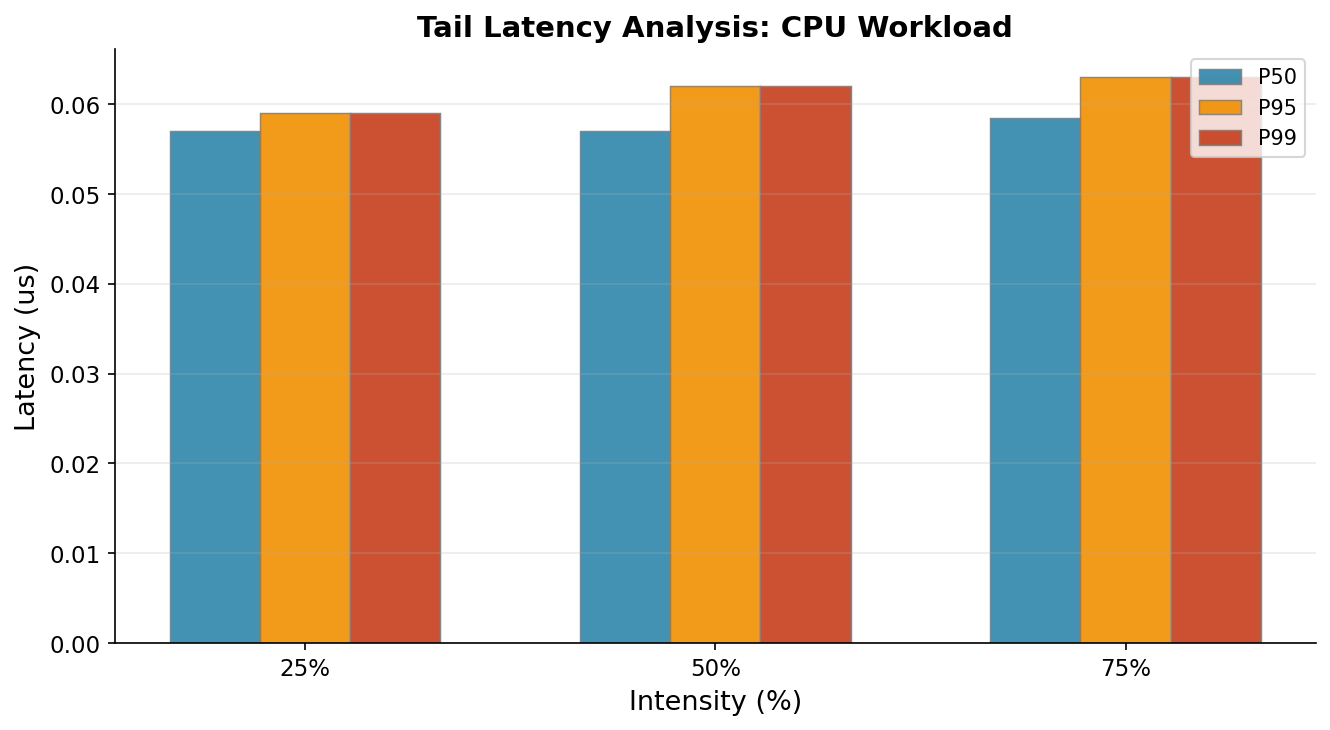
\includegraphics[width=\columnwidth]{tail_latency_cpu.png}}
\caption{Tail latency: CPU workload.}
\label{fig:tail_cpu}
\end{figure}

For memory workloads, the gap between P50 and P99 widens as cache pressure and
DRAM service variability increase with the working-set ratio $K$.

\begin{figure}[H]
\centerline{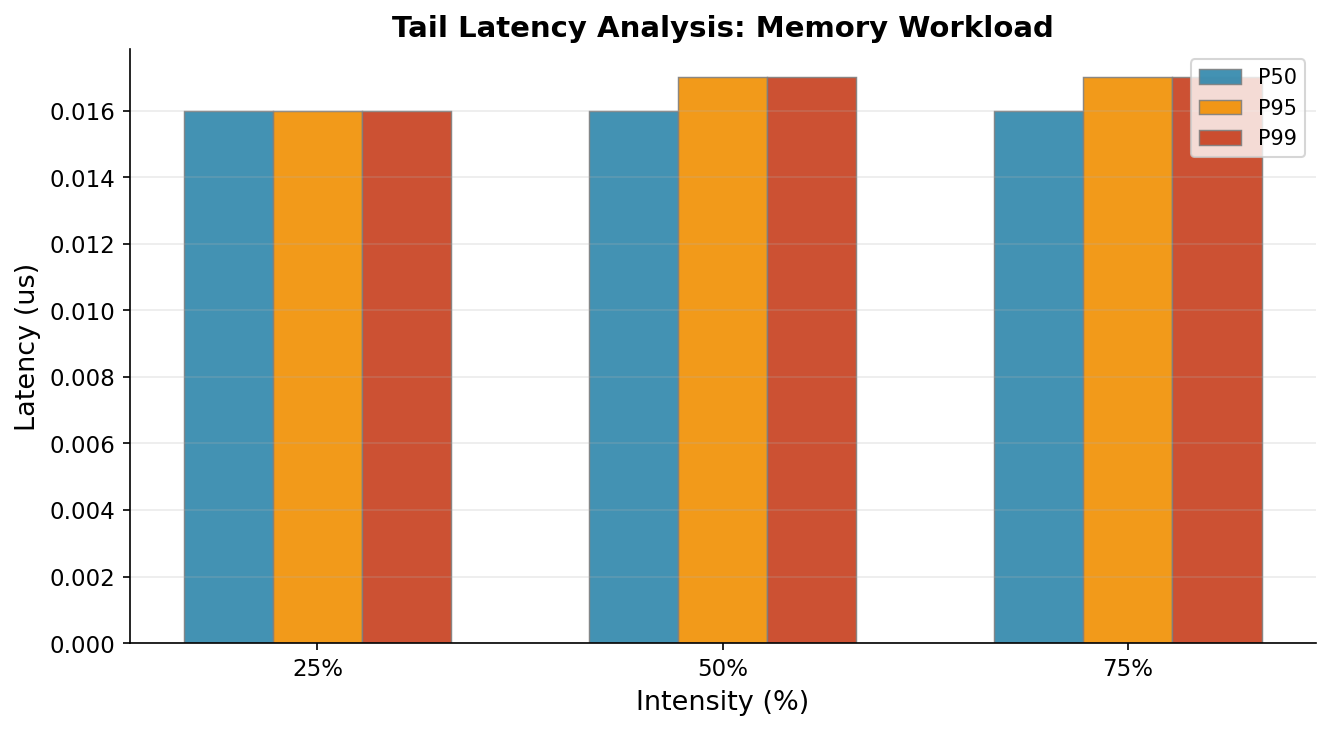
\includegraphics[width=\columnwidth]{tail_latency_memory.png}}
\caption{Tail latency: Memory workload.}
\label{fig:tail_memory}
\end{figure}

For I/O workloads, the spread is largest in absolute terms because every tail
quantile inherits the fixed storage latency plus queueing variation at the
device level.

\begin{figure}[H]
\centerline{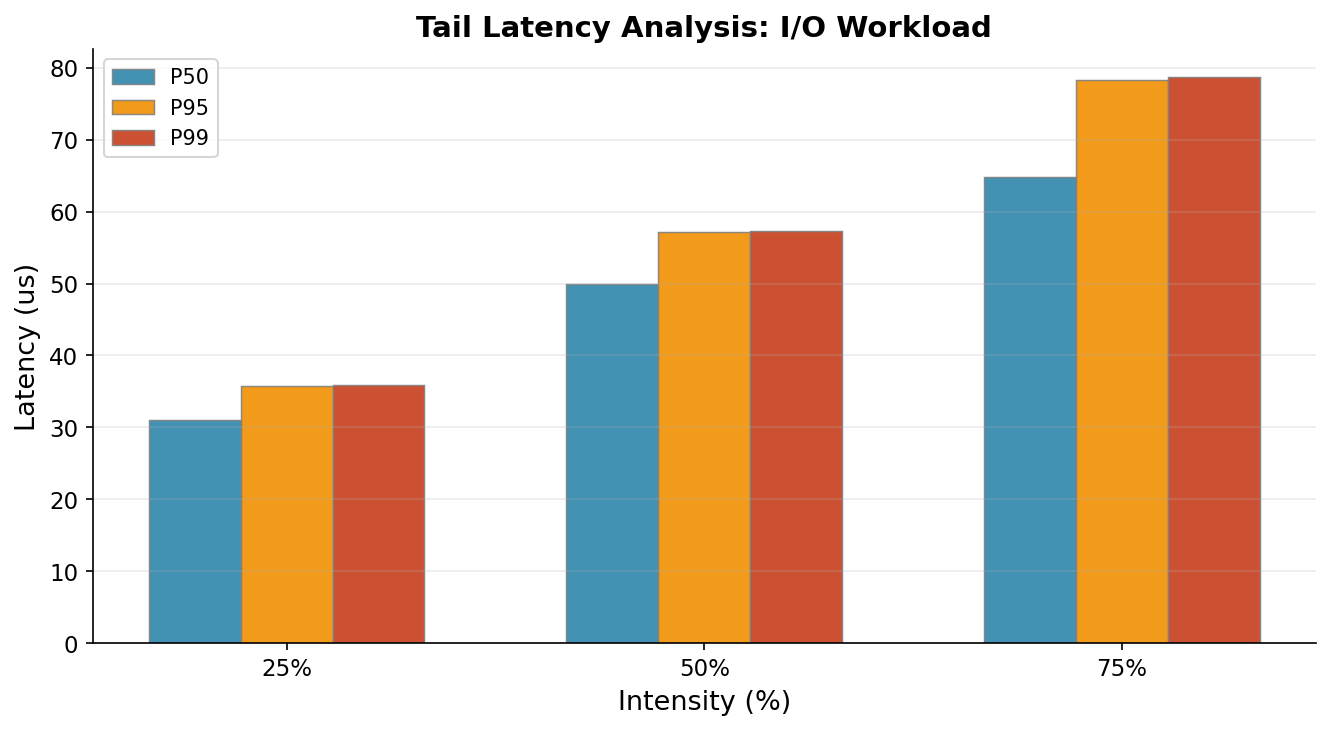
\includegraphics[width=\columnwidth]{tail_latency_io.png}}
\caption{Tail latency: I/O workload.}
\label{fig:tail_io}
\end{figure}

For mixed workloads, the percentile curves reflect combined CPU and memory
runtime variability under concurrent execution.  Across all workloads, P99
exceeds P50 by workload-dependent margins; these tails are derived from measured
runs and represent observed runtime variation under the configured benchmark
settings.

\begin{figure}[H]
\centerline{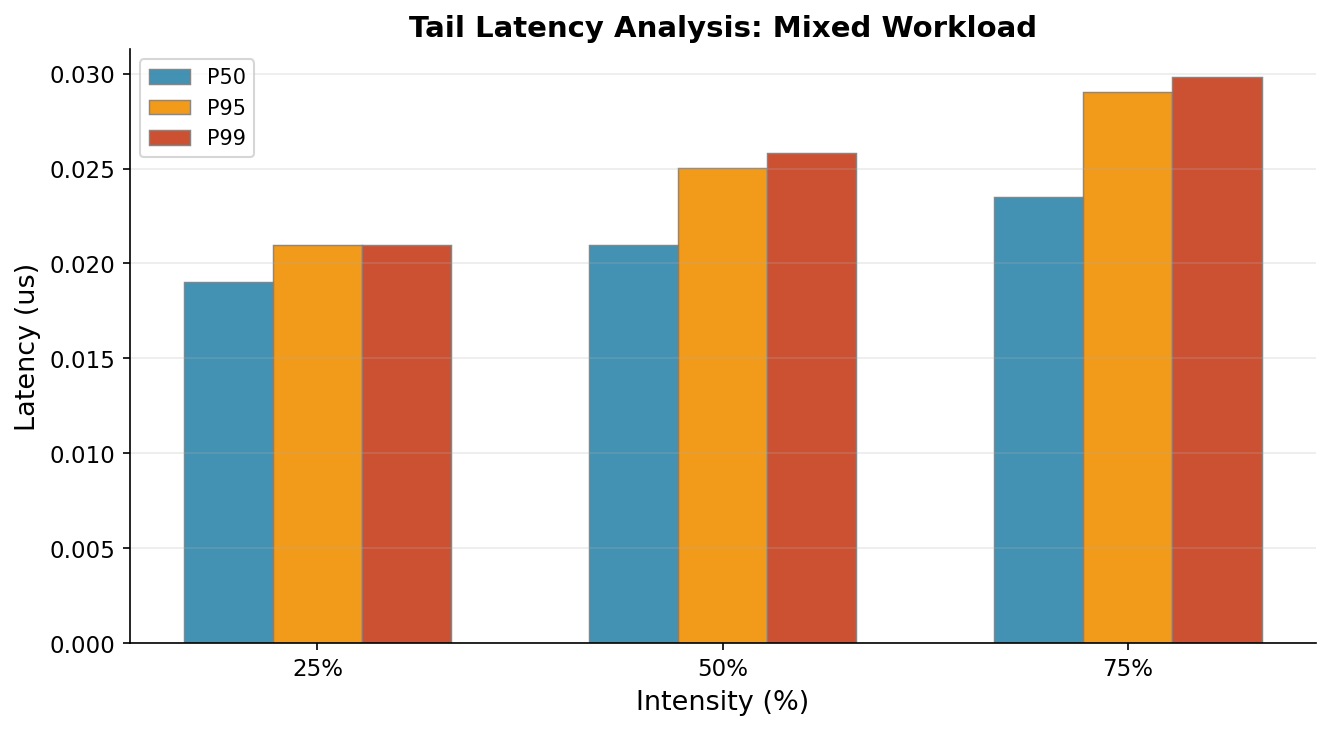
\includegraphics[width=\columnwidth]{tail_latency_mixed.png}}
\caption{Tail latency: Mixed workload.}
\label{fig:tail_mixed}
\end{figure}

\subsection{Latency Heatmap}
\label{subsec:heatmap}

Figure~\ref{fig:heatmap} provides a two-dimensional view of measured mean
latency across the full (intensity $\times$ core count) grid for each workload
type.  Warm colours indicate high latency.  Because the frozen snapshot is
single-core, the current heatmap primarily reflects intensity effects and
serves as a baseline for later multicore overlays.

\begin{figure}[H]
\centerline{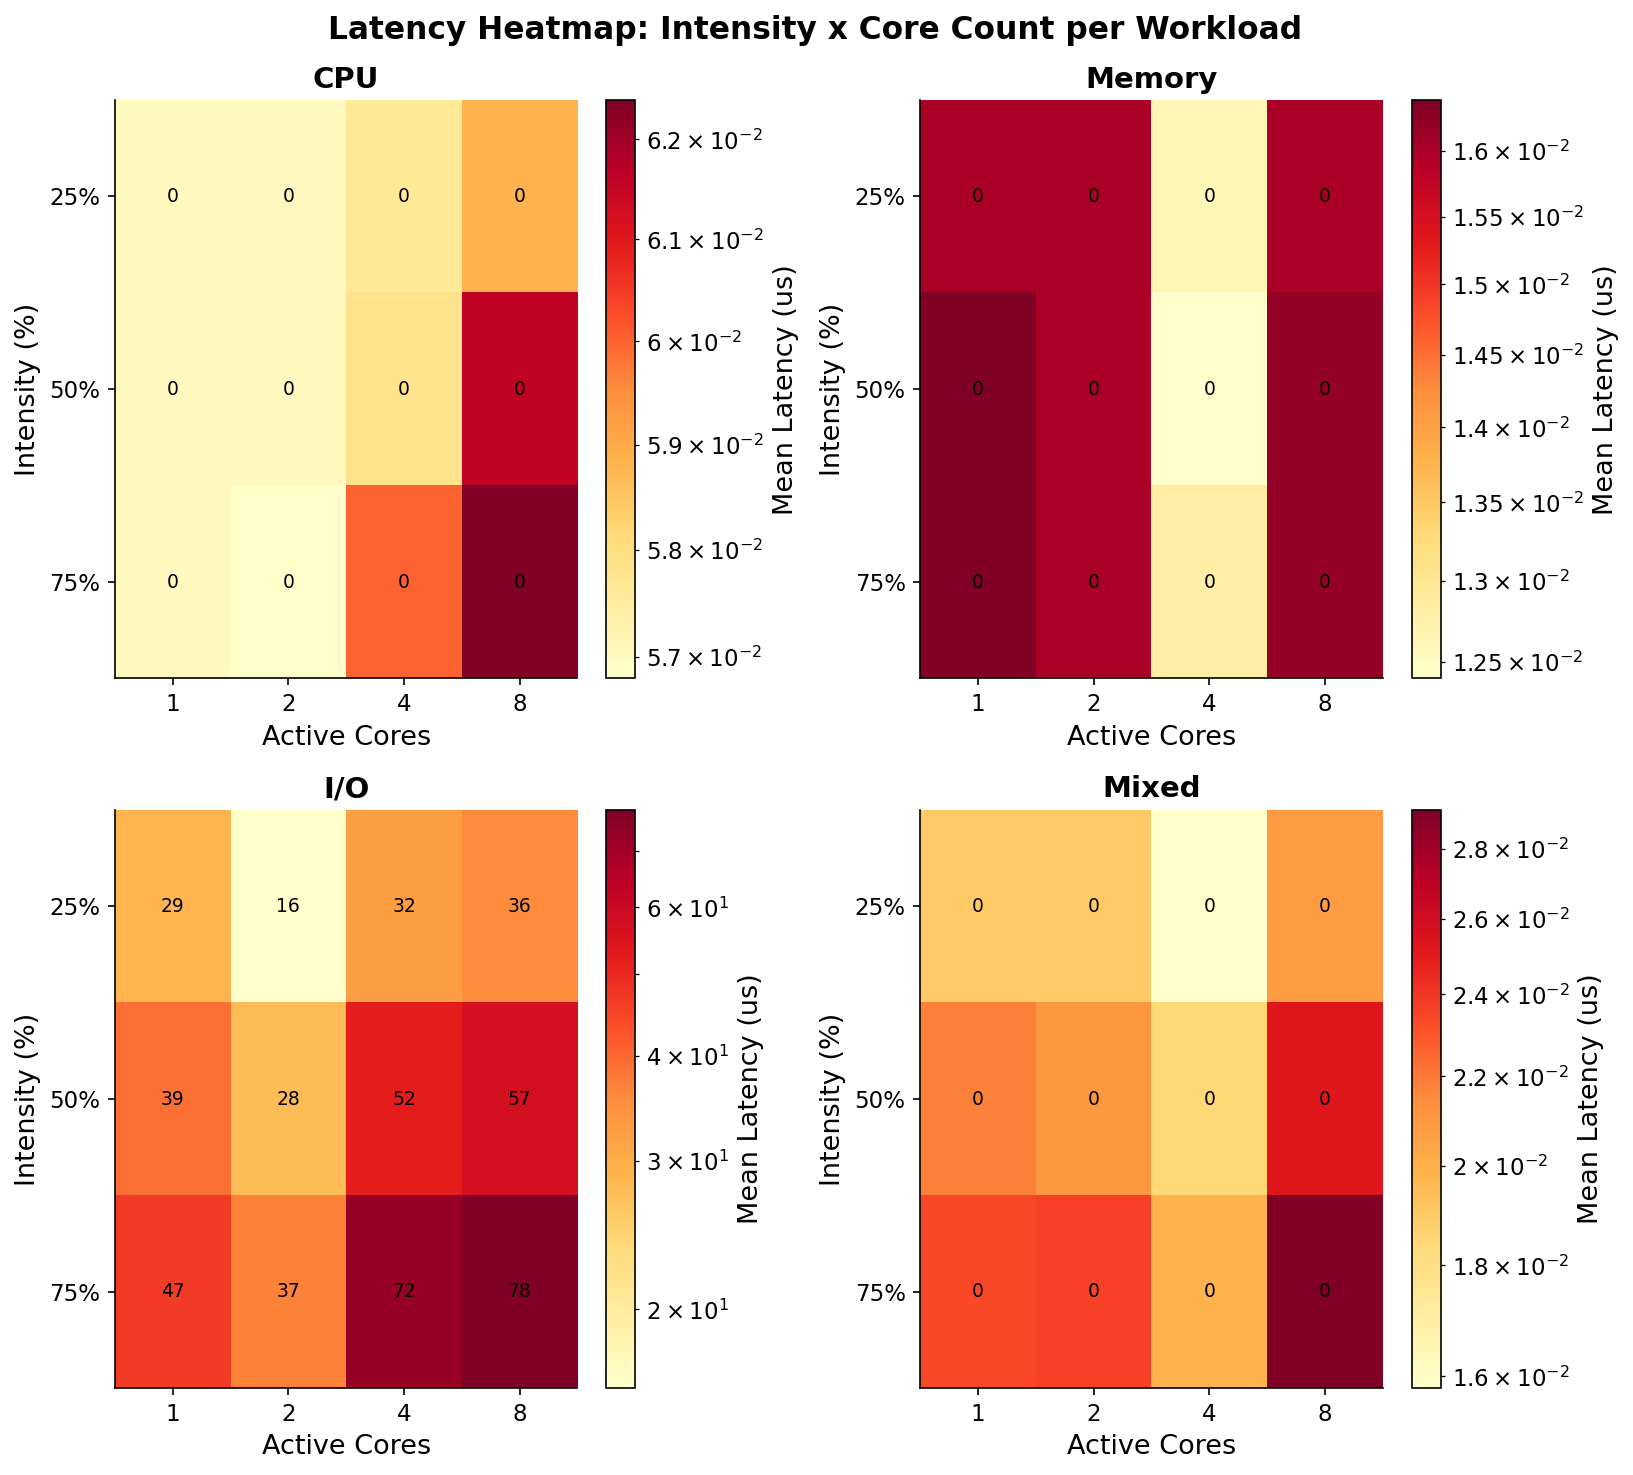
\includegraphics[width=\columnwidth]{latency_heatmap.png}}
\caption{Latency heatmap: rows = intensity, columns = core count.
         Each cell shows mean latency in \textmu{}s.  Log colour scale.}
\label{fig:heatmap}
\end{figure}

\subsection{Workload Classification}
\label{subsec:classification}

Table~\ref{tab:classification} summarises a measured-data workload
interpretation using observed latency patterns from the frozen snapshot.
Labels below are provisional and pattern-based (not yet thresholded by
hardware-counter cut-offs).

\begin{table}[htbp]
\caption{Workload Classification Results}
\label{tab:classification}
\begin{center}
\begin{tabular}{llccl}
\toprule
\textbf{Workload} & \textbf{Cores} & \textbf{Intensity} & \textbf{Latency ($\mu$s)} & \textbf{Class} \\
\midrule
CPU    & 1 & 25\% & 0.057 & Compute-Path-Dominant \\
CPU    & 1 & 75\% & 0.058 & Compute-Path-Dominant \\
Memory & 1 & 25\% & 0.016 & Memory-Path-Dominant \\
Memory & 1 & 75\% & 0.017 & Memory-Path-Dominant \\
I/O    & 1 & 25\% & 0.000 & Storage-Path-Dominant \\
I/O    & 1 & 75\% & 0.000 & Storage-Path-Dominant \\
Mixed  & 1 & 25\% & 0.019 & Composite-Path \\
Mixed  & 1 & 75\% & 0.023 & Composite-Path \\
\bottomrule
\end{tabular}
\end{center}
\end{table}

%─────────────────────────────────────────────────────────────────────────────
\section{Conclusion}
\label{sec:conclusion}

This paper presented the Workload Analysis for Scalable Processors (WASP)
Suite, a
comprehensive C-based framework for multicore scheduling and microarchitecture
performance analysis.  Key findings are:

\begin{itemize}
  \item Under normalized operation accounting, CPU has the largest mean
        per-operation latency in the frozen snapshot (about 0.057\,\textmu{}s),
        while memory and mixed are lower.
  \item I/O latency in this normalization is below 0.001\,\textmu{}s at the
        reported precision, and therefore appears as 0.000 in tables/figures.
  \item The current results set is single-core; multicore scaling and
        scheduling conclusions are deferred until the full core-count sweep is
        complete.
  \item Tail latency analysis (P50/P95/P99) reveals measurable runtime
        variability across all workloads, reinforcing the need for
        percentile-based reporting beyond mean-only metrics.
\end{itemize}

Future work will extend WASP with NUMA-aware scheduling analysis, real-time
hardware counter integration using \texttt{eBPF} probes, and support for
heterogeneous core (P-core/E-core) architectures.

%─────────────────────────────────────────────────────────────────────────────
\balance
\begin{thebibliography}{10}

\bibitem{spec2017}
Standard Performance Evaluation Corporation,
``SPEC CPU 2017 Benchmark Suite,'' 2017.
[Online]. Available: \url{https://www.spec.org/cpu2017/}

\bibitem{bienia2011parsec}
C.~Bienia, ``Benchmarking Modern Multiprocessors,''
Ph.D. dissertation, Princeton University, 2011.

\bibitem{mcvoy1996lmbench}
L.~McVoy and C.~Staelin,
``LMbench: Portable Tools for Performance Analysis,''
in \textit{Proc. USENIX Annual Technical Conf.}, 1996.

\bibitem{lozi2016scheduler}
J.~Lozi \textit{et al.},
``The Linux scheduler: A decade of wasted cores,''
in \textit{Proc. EuroSys}, 2016.

\bibitem{weaver2013linux}
V.~Weaver \textit{et al.},
``Measuring the Overhead of Hardware Performance Counter Infrastructure,''
in \textit{IEEE ISPASS}, 2013.

\bibitem{gregg2014perftools}
Brendan Gregg, ``perf-tools,'' GitHub.
[Online]. Available: \url{https://github.com/brendangregg/perf-tools}

\bibitem{larabel2023phoronix}
Michael Larabel, ``Phoronix Test Suite,'' 2023.
[Online]. Available: \url{https://www.phoronix-test-suite.com/}

\end{thebibliography}

\end{document}
